\chapter{Algoritmos de string}

Este capítulo aborda algoritmos eficientes para processamento de strings. Muitos problemas de string podem ser facilmente resolvidos em tempo $O(n^2)$, mas o desafio é encontrar algoritmos que funcionem em tempo $O(n)$ ou $O(n \log n)$.

\index{pattern matching}

Por exemplo, um problema fundamental de processamento de strings é o problema de \key{casamento de padrão}: dada uma string de comprimento $n$ e um padrão de comprimento $m$, nossa tarefa é encontrar as ocorrências do padrão na string. Por exemplo, o padrão \texttt{ABC} ocorre duas vezes na string \texttt{ABABCBABC}.

O problema de casamento de padrão pode ser facilmente resolvido em tempo $O(nm)$ por um algoritmo de força bruta que testa todas as posições onde o padrão pode ocorrer na string. No entanto, neste capítulo, veremos que existem algoritmos mais eficientes que requerem apenas tempo $O(n+m)$.

\index{string}

\section{Terminologia de string}

\index{alphabet}

Ao longo do capítulo, assumimos que a indexação baseada em zero é usada em strings. Assim, uma string \texttt{s} de comprimento $n$ consiste nos caracteres $\texttt{s}[0],\texttt{s}[1],\ldots,\texttt{s}[n-1]$. O conjunto de caracteres que podem aparecer em strings é chamado de \key{alfabeto}. Por exemplo, o alfabeto $\{\texttt{A},\texttt{B},\ldots,\texttt{Z}\}$ consiste nas letras maiúsculas do inglês.

\index{substring}

Uma \key{substring} é uma sequência de caracteres consecutivos em uma string. Usamos a notação $\texttt{s}[a \ldots b]$ para nos referir a uma substring de \texttt{s} que começa na posição $a$ e termina na posição $b$. Uma string de comprimento $n$ possui $n(n+1)/2$ substrings. Por exemplo, as substrings de \texttt{ABCD} são \texttt{A}, \texttt{B}, \texttt{C}, \texttt{D}, \texttt{AB}, \texttt{BC}, \texttt{CD}, \texttt{ABC}, \texttt{BCD} e \texttt{ABCD}.

\index{subsequence}

Uma \key{subsequência} é uma sequência de caracteres (não necessariamente consecutivos) em uma string em sua ordem original. Uma string de comprimento $n$ possui $2^n-1$ subsequências. Por exemplo, as subsequências de \texttt{ABCD} são \texttt{A}, \texttt{B}, \texttt{C}, \texttt{D}, \texttt{AB}, \texttt{AC}, \texttt{AD}, \texttt{BC}, \texttt{BD}, \texttt{CD}, \texttt{ABC}, \texttt{ABD}, \texttt{ACD}, \texttt{BCD} e \texttt{ABCD}.

\index{prefix}
\index{suffix}

Um \key{prefixo} é uma substring que começa no início de uma string, e um \key{sufixo} é uma substring que termina no final de uma string. Por exemplo, os prefixos de \texttt{ABCD} são \texttt{A}, \texttt{AB}, \texttt{ABC} e \texttt{ABCD}, e os sufixos de \texttt{ABCD} são \texttt{D}, \texttt{CD}, \texttt{BCD} e \texttt{ABCD}.

\index{rotation}

Uma \key{rotação} pode ser gerada movendo os caracteres de uma string um por um do início para o final (ou vice-versa). Por exemplo, as rotações de \texttt{ABCD} são \texttt{ABCD}, \texttt{BCDA}, \texttt{CDAB} e \texttt{DABC}.

\index{period}

Um \key{período} é um prefixo de uma string tal que a string pode ser construída repetindo o período. A última repetição pode ser parcial e conter apenas um prefixo do período. Por exemplo, o menor período de \texttt{ABCABCA} é \texttt{ABC}.

\index{border}

Uma \key{borda} é uma string que é tanto um prefixo quanto um sufixo de uma string. Por exemplo, as bordas de \texttt{ABACABA} são \texttt{A}, \texttt{ABA} e \texttt{ABACABA}.

\index{lexicographical order}

As strings são comparadas usando a \key{ordem lexicográfica} (que corresponde à ordem alfabética). Isso significa que $x<y$ se $x \neq y$ e $x$ é um prefixo de $y$, ou existe uma posição $k$ tal que $x[i]=y[i]$ quando $i<k$ e $x[k]<y[k]$.

\section{Estrutura Trie}

\index{trie}

Uma \key{trie} é uma árvore enraizada que mantém um conjunto de strings. Cada string no conjunto é armazenada como uma cadeia de caracteres que começa na raiz. Se duas strings tiverem um prefixo comum, elas também terão uma cadeia comum na árvore.

Por exemplo, considere a seguinte trie:

\begin{center}
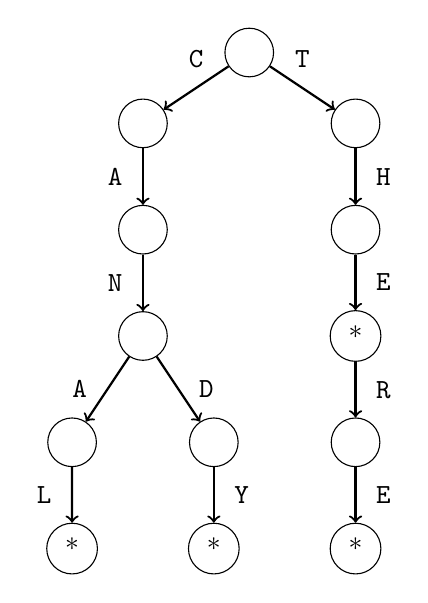
\begin{tikzpicture}[scale=0.9]
\node[draw, circle] (1) at (0,20) {$\phantom{1}$};
\node[draw, circle] (2) at (-1.5,19) {$\phantom{1}$};
\node[draw, circle] (3) at (1.5,19) {$\phantom{1}$};
\node[draw, circle] (4) at (-1.5,17.5) {$\phantom{1}$};
\node[draw, circle] (5) at (-1.5,16) {$\phantom{1}$};
\node[draw, circle] (6) at (-2.5,14.5) {$\phantom{1}$};
\node[draw, circle] (7) at (-0.5,14.5) {$\phantom{1}$};
\node[draw, circle] (8) at (-2.5,13) {*};
\node[draw, circle] (9) at (-0.5,13) {*};
\node[draw, circle] (10) at (1.5,17.5) {$\phantom{1}$};
\node[draw, circle] (11) at (1.5,16) {*};
\node[draw, circle] (12) at (1.5,14.5) {$\phantom{1}$};
\node[draw, circle] (13) at (1.5,13) {*};

\path[draw,thick,->] (1) -- node[font=\small,label=\texttt{C}] {} (2);
\path[draw,thick,->] (1) -- node[font=\small,label=\texttt{T}] {} (3);
\path[draw,thick,->] (2) -- node[font=\small,label=left:\texttt{A}] {} (4);
\path[draw,thick,->] (4) -- node[font=\small,label=left:\texttt{N}] {} (5);
\path[draw,thick,->] (5) -- node[font=\small,label=left:\texttt{A}] {} (6);
\path[draw,thick,->] (5) -- node[font=\small,label=right:\texttt{D}] {} (7);
\path[draw,thick,->] (6) -- node[font=\small,label=left:\texttt{L}] {}(8);
\path[draw,thick,->] (7) -- node[font=\small,label=right:\texttt{Y}] {} (9);
\path[draw,thick,->] (3) -- node[font=\small,label=right:\texttt{H}] {} (10);
\path[draw,thick,->] (10) -- node[font=\small,label=right:\texttt{E}] {} (11);
\path[draw,thick,->] (11) -- node[font=\small,label=right:\texttt{R}] {} (12);
\path[draw,thick,->] (12) -- node[font=\small,label=right:\texttt{E}] {} (13);
\end{tikzpicture}
\end{center}

Esta trie corresponde ao conjunto $\{\texttt{CANAL},\texttt{CANDY},\texttt{THE},\texttt{THERE}\}$. O caractere * em um nó significa que uma string no conjunto termina naquele nó. Esse caractere é necessário porque uma string pode ser um prefixo de outra string. Por exemplo, na trie acima, \texttt{THE} é um prefixo de \texttt{THERE}.

Podemos verificar em tempo $O(n)$ se uma trie contém uma string de comprimento $n$, porque podemos seguir a cadeia que começa no nó raiz. Também podemos adicionar uma string de comprimento $n$ à trie em tempo $O(n)$ seguindo primeiro a cadeia e depois adicionando novos nós à trie, se necessário.

Usando uma trie, podemos encontrar o prefixo mais longo de uma determinada string tal que o prefixo pertence ao conjunto. Além disso, armazenando informações adicionais em cada nó, podemos calcular o número de strings que pertencem ao conjunto e têm uma determinada string como prefixo.

Uma trie pode ser armazenada em um array
\begin{lstlisting}
int trie[N][A];
\end{lstlisting}
onde $N$ é o número máximo de nós (o comprimento total máximo das strings no conjunto) e $A$ é o tamanho do alfabeto. Os nós de uma trie são numerados $0,1,2,\ldots$ de forma que o número da raiz seja 0, e $\texttt{trie}[s][c]$ é o próximo nó na cadeia quando nos movemos do nó $s$ usando o caractere $c$.

\section{Hashing de string}

\index{hashing}
\index{string hashing}

\key{Hashing de string} é uma técnica que nos permite verificar eficientemente se duas strings são iguais\footnote{A técnica foi popularizada pelo algoritmo de casamento de padrão Karp–Rabin \cite{kar87}.}. A ideia no hashing de string é comparar valores de hash de strings em vez de seus caracteres individuais.

\subsubsection*{Calculando valores de hash}

\index{hash value}
\index{polynomial hashing}

Um \key{valor de hash} de uma string é um número que é calculado a partir dos caracteres da string. Se duas strings são iguais, seus valores de hash também são iguais, o que torna possível comparar strings com base em seus valores de hash.

Uma maneira usual de implementar hashing de string é o \key{hashing polinomial}, o que significa que o valor de hash de uma string \texttt{s} de comprimento $n$ é 
\[(\texttt{s}[0] A^{n-1} + \texttt{s}[1] A^{n-2} + \cdots + \texttt{s}[n-1] A^0) \bmod B  ,\]
onde $s[0],s[1],\ldots,s[n-1]$ são interpretados como os códigos dos caracteres de \texttt{s}, e $A$ e $B$ são constantes pré-escolhidas.

Por exemplo, os códigos dos caracteres de \texttt{ALLEY} são:
\begin{center}
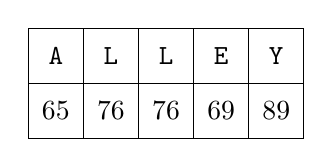
\begin{tikzpicture}[scale=0.7]
\draw (0,0) grid (5,2);

\node at (0.5, 1.5) {\texttt{A}};
\node at (1.5, 1.5) {\texttt{L}};
\node at (2.5, 1.5) {\texttt{L}};
\node at (3.5, 1.5) {\texttt{E}};
\node at (4.5, 1.5) {\texttt{Y}};

\node at (0.5, 0.5) {65};
\node at (1.5, 0.5) {76};
\node at (2.5, 0.5) {76};
\node at (3.5, 0.5) {69};
\node at (4.5, 0.5) {89};

\end{tikzpicture}
\end{center}

Assim, se $A=3$ e $B=97$, o valor de hash de \texttt{ALLEY} é
\[(65 \cdot 3^4 + 76 \cdot 3^3 + 76 \cdot 3^2 + 69 \cdot 3^1 + 89 \cdot 3^0) \bmod 97 = 52.\]

\subsubsection*{Pré-processamento}

Usando hashing polinomial, podemos calcular o valor de hash de qualquer substring de uma string \texttt{s} em tempo $O(1)$ após um pré-processamento de tempo $O(n)$. A ideia é construir um array \texttt{h} tal que $\texttt{h}[k]$ contenha o valor de hash do prefixo $\texttt{s}[0 \ldots k]$. Os valores do array podem ser calculados recursivamente da seguinte forma:
\[
\begin{array}{lcl}
\texttt{h}[0] & = & \texttt{s}[0] \\
\texttt{h}[k] & = & (\texttt{h}[k-1] A + \texttt{s}[k]) \bmod B \\
\end{array}
\]
Além disso, construímos um array $\texttt{p}$ onde $\texttt{p}[k]=A^k \bmod B$:
\[
\begin{array}{lcl}
\texttt{p}[0] & = & 1 \\
\texttt{p}[k] & = & (\texttt{p}[k-1] A) \bmod B. \\
\end{array}
\]
Construir esses arrays leva tempo $O(n)$. Depois disso, o valor de hash de qualquer substring $\texttt{s}[a \ldots b]$ pode ser calculado em tempo $O(1)$ usando a fórmula
\[(\texttt{h}[b]-\texttt{h}[a-1] \texttt{p}[b-a+1]) \bmod B\]
assumindo que $a>0$. Se $a=0$, o valor de hash é simplesmente $\texttt{h}[b]$.

\subsubsection*{Usando valores de hash}

Podemos comparar strings de forma eficiente usando valores de hash. Em vez de comparar os caracteres individuais das strings, a ideia é comparar seus valores de hash. Se os valores de hash forem iguais, as strings são \emph{provavelmente} iguais, e se os valores de hash forem diferentes, as strings são \emph{certamente} diferentes.

Usando hashing, podemos frequentemente tornar um algoritmo de força bruta eficiente. Como exemplo, considere o problema de casamento de padrão: dada uma string $s$ e um padrão $p$, encontre as posições onde $p$ ocorre em $s$. Um algoritmo de força bruta percorre todas as posições onde $p$ pode ocorrer e compara as strings caractere por caractere. A complexidade de tempo de tal algoritmo é $O(n^2)$.

Podemos tornar o algoritmo de força bruta mais eficiente usando hashing, porque o algoritmo compara substrings de strings. Usando hashing, cada comparação leva apenas tempo $O(1)$, porque apenas valores de hash de substrings são comparados. Isso resulta em um algoritmo com complexidade de tempo $O(n)$, que é a melhor complexidade de tempo possível para este problema.

Combinando hashing e \emph{busca binária}, também é possível descobrir a ordem lexicográfica de duas strings em tempo logarítmico. Isso pode ser feito calculando o comprimento do prefixo comum das strings usando busca binária. Uma vez que sabemos o comprimento do prefixo comum, podemos apenas verificar o próximo caractere após o prefixo, porque isso determina a ordem das strings.

\subsubsection*{Colisões e parâmetros}

\index{collision}

Um risco evidente ao comparar valores de hash é uma \key{colisão}, o que significa que duas strings têm conteúdo diferente, mas valores de hash iguais. Nesse caso, um algoritmo que se baseia nos valores de hash conclui que as strings são iguais, mas na realidade não são, e o algoritmo pode fornecer resultados incorretos.

Colisões são sempre possíveis, porque o número de strings diferentes é maior que o número de valores de hash diferentes. No entanto, a probabilidade de uma colisão é pequena se as constantes $A$ e $B$ forem cuidadosamente escolhidas. Uma maneira usual é escolher constantes aleatórias próximas a $10^9$, por exemplo, da seguinte forma:
\[
\begin{array}{lcl}
A & = & 911382323 \\
B & = & 972663749 \\
\end{array}
\]

Usando tais constantes, o tipo \texttt{long long} pode ser usado ao calcular valores de hash, porque os produtos $AB$ e $BB$ caberão em \texttt{long long}. Mas é suficiente ter cerca de $10^9$ valores de hash diferentes?

Vamos considerar três cenários onde o hashing pode ser usado:

\textit{Cenário 1:} As strings $x$ e $y$ são comparadas entre si. A probabilidade de uma colisão é $1/B$, assumindo que todos os valores de hash são igualmente prováveis.

\textit{Cenário 2:} Uma string $x$ é comparada com as strings $y_1,y_2,\ldots,y_n$. A probabilidade de uma ou mais colisões é

\[1-(1-\frac{1}{B})^n.\]

\textit{Cenário 3:} Todos os pares de strings $x_1,x_2,\ldots,x_n$ são comparados entre si. A probabilidade de uma ou mais colisões é
\[ 1 - \frac{B \cdot (B-1) \cdot (B-2) \cdots (B-n+1)}{B^n}.\]

A tabela a seguir mostra as probabilidades de colisão quando $n=10^6$ e o valor de $B$ varia:

\begin{center}
\begin{tabular}{rrrr}
constante $B$ & cenário 1 & cenário 2 & cenário 3 \\
\hline
$10^3$ & $0.001000$ & $1.000000$ & $1.000000$ \\
$10^6$ & $0.000001$ & $0.632121$ & $1.000000$ \\
$10^9$ & $0.000000$ & $0.001000$ & $1.000000$ \\
$10^{12}$ & $0.000000$ & $0.000000$ & $0.393469$ \\
$10^{15}$ & $0.000000$ & $0.000000$ & $0.000500$ \\
$10^{18}$ & $0.000000$ & $0.000000$ & $0.000001$ \\
\end{tabular}
\end{center}

A tabela mostra que, no cenário 1, a probabilidade de uma colisão é desprezível quando $B \approx 10^9$. No cenário 2, uma colisão é possível, mas a probabilidade ainda é muito pequena. No entanto, no cenário 3, a situação é muito diferente: uma colisão quase sempre acontecerá quando $B \approx 10^9$.

\index{birthday paradox}

O fenômeno no cenário 3 é conhecido como o \key{paradoxo do aniversário}: se houver $n$ pessoas em uma sala, a probabilidade de \emph{algumas} duas pessoas fazerem aniversário no mesmo dia é grande mesmo que $n$ seja muito pequeno. No hashing, da mesma forma, quando todos os valores de hash são comparados entre si, a probabilidade de que dois valores de hash sejam iguais é grande.

Podemos diminuir a probabilidade de uma colisão calculando \emph{múltiplos} valores de hash usando parâmetros diferentes. É improvável que uma colisão ocorra em todos os valores de hash ao mesmo tempo. Por exemplo, dois valores de hash com parâmetro $B \approx 10^9$ correspondem a um valor de hash com parâmetro $B \approx 10^{18}$, o que torna a probabilidade de uma colisão muito pequena.

Algumas pessoas usam constantes $B=2^{32}$ e $B=2^{64}$, o que é conveniente, porque as operações com inteiros de 32 e 64 bits são calculadas módulo $2^{32}$ e $2^{64}$. No entanto, esta \emph{não} é uma boa escolha, porque é possível construir entradas que sempre geram colisões quando constantes da forma $2^x$ são usadas \cite{pac13}.

\section{Algoritmo Z}

\index{Z-algorithm}
\index{Z-array}

O \key{array Z} \texttt{z} de uma string \texttt{s} de comprimento $n$ contém para cada $k=0,1,\ldots,n-1$ o comprimento da substring mais longa de \texttt{s} que começa na posição $k$ e é um prefixo de \texttt{s}. Assim, $\texttt{z}[k]=p$ nos diz que $\texttt{s}[0 \ldots p-1]$ é igual a $\texttt{s}[k \ldots k+p-1]$. Muitos problemas de processamento de strings podem ser resolvidos de forma eficiente usando o array Z.

Por exemplo, o array Z de \texttt{ACBACDACBACBACDA} é o seguinte:

\begin{center}
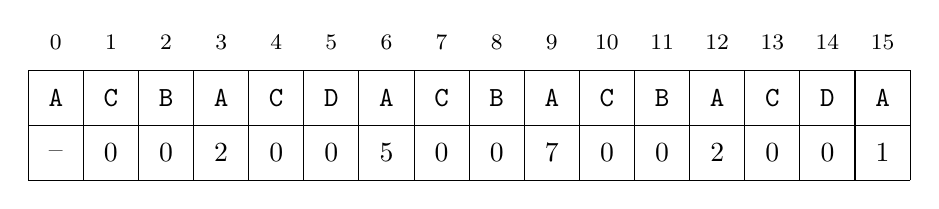
\begin{tikzpicture}[scale=0.7]
\draw (0,0) grid (16,2);

\node at (0.5, 1.5) {\texttt{A}};
\node at (1.5, 1.5) {\texttt{C}};
\node at (2.5, 1.5) {\texttt{B}};
\node at (3.5, 1.5) {\texttt{A}};
\node at (4.5, 1.5) {\texttt{C}};
\node at (5.5, 1.5) {\texttt{D}};
\node at (6.5, 1.5) {\texttt{A}};
\node at (7.5, 1.5) {\texttt{C}};
\node at (8.5, 1.5) {\texttt{B}};
\node at (9.5, 1.5) {\texttt{A}};
\node at (10.5, 1.5) {\texttt{C}};
\node at (11.5, 1.5) {\texttt{B}};
\node at (12.5, 1.5) {\texttt{A}};
\node at (13.5, 1.5) {\texttt{C}};
\node at (14.5, 1.5) {\texttt{D}};
\node at (15.5, 1.5) {\texttt{A}};

\node at (0.5, 0.5) {--};
\node at (1.5, 0.5) {0};
\node at (2.5, 0.5) {0};
\node at (3.5, 0.5) {2};
\node at (4.5, 0.5) {0};
\node at (5.5, 0.5) {0};
\node at (6.5, 0.5) {5};
\node at (7.5, 0.5) {0};
\node at (8.5, 0.5) {0};
\node at (9.5, 0.5) {7};
\node at (10.5, 0.5) {0};
\node at (11.5, 0.5) {0};
\node at (12.5, 0.5) {2};
\node at (13.5, 0.5) {0};
\node at (14.5, 0.5) {0};
\node at (15.5, 0.5) {1};

\footnotesize
\node at (0.5, 2.5) {0};
\node at (1.5, 2.5) {1};
\node at (2.5, 2.5) {2};
\node at (3.5, 2.5) {3};
\node at (4.5, 2.5) {4};
\node at (5.5, 2.5) {5};
\node at (6.5, 2.5) {6};
\node at (7.5, 2.5) {7};
\node at (8.5, 2.5) {8};
\node at (9.5, 2.5) {9};
\node at (10.5, 2.5) {10};
\node at (11.5, 2.5) {11};
\node at (12.5, 2.5) {12};
\node at (13.5, 2.5) {13};
\node at (14.5, 2.5) {14};
\node at (15.5, 2.5) {15};

\end{tikzpicture}
\end{center}

Neste caso, por exemplo, $\texttt{z}[6]=5$, porque a substring \texttt{ACBAC} de comprimento 5 é um prefixo de \texttt{s}, mas a substring \texttt{ACBACB} de comprimento 6 não é um prefixo de \texttt{s}.

\subsubsection*{Descrição do algoritmo}

A seguir, descrevemos um algoritmo, chamado de \key{algoritmo Z}\footnote{O algoritmo Z foi apresentado em \cite{gus97} como o método mais simples conhecido para casamento de padrão em tempo linear, e a ideia original foi atribuída a \cite{mai84}.}, que constrói eficientemente o array Z em tempo $O(n)$. O algoritmo calcula os valores do array Z da esquerda para a direita, usando informações já armazenadas no array Z e comparando substrings caractere por caractere.

Para calcular os valores do array Z de forma eficiente, o algoritmo mantém um intervalo $[x,y]$ tal que $\texttt{s}[x \ldots y]$ é um prefixo de \texttt{s} e $y$ é o maior possível. Como sabemos que $\texttt{s}[0 \ldots y-x]$ e $\texttt{s}[x \ldots y]$ são iguais, podemos usar essa informação ao calcular os valores Z para as posições $x+1,x+2,\ldots,y$.

Em cada posição $k$, primeiro verificamos o valor de $\texttt{z}[k-x]$. Se $k+\texttt{z}[k-x]<y$, sabemos que $\texttt{z}[k]=\texttt{z}[k-x]$. No entanto, se $k+\texttt{z}[k-x] \ge y$, $\texttt{s}[0 \ldots y-k]$ é igual a $\texttt{s}[k \ldots y]$, e para determinar o valor de $\texttt{z}[k]$ precisamos comparar as substrings caractere por caractere. Ainda assim, o algoritmo funciona em tempo $O(n)$, porque começamos a comparar nas posições $y-k+1$ e $y+1$.

Por exemplo, vamos construir o seguinte array Z:

\begin{center}
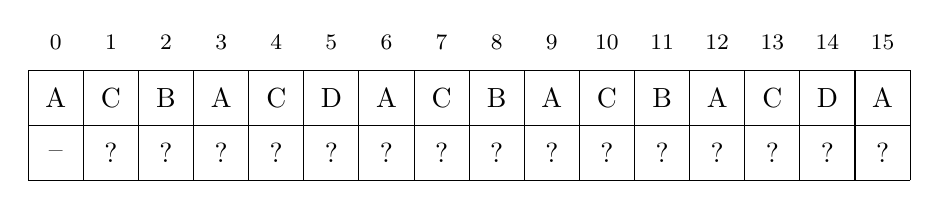
\begin{tikzpicture}[scale=0.7]
\draw (0,0) grid (16,2);

\node at (0.5, 1.5) {A};
\node at (1.5, 1.5) {C};
\node at (2.5, 1.5) {B};
\node at (3.5, 1.5) {A};
\node at (4.5, 1.5) {C};
\node at (5.5, 1.5) {D};
\node at (6.5, 1.5) {A};
\node at (7.5, 1.5) {C};
\node at (8.5, 1.5) {B};
\node at (9.5, 1.5) {A};
\node at (10.5, 1.5) {C};
\node at (11.5, 1.5) {B};
\node at (12.5, 1.5) {A};
\node at (13.5, 1.5) {C};
\node at (14.5, 1.5) {D};
\node at (15.5, 1.5) {A};

\node at (0.5, 0.5) {--};
\node at (1.5, 0.5) {?};
\node at (2.5, 0.5) {?};
\node at (3.5, 0.5) {?};
\node at (4.5, 0.5) {?};
\node at (5.5, 0.5) {?};
\node at (6.5, 0.5) {?};
\node at (7.5, 0.5) {?};
\node at (8.5, 0.5) {?};
\node at (9.5, 0.5) {?};
\node at (10.5, 0.5) {?};
\node at (11.5, 0.5) {?};
\node at (12.5, 0.5) {?};
\node at (13.5, 0.5) {?};
\node at (14.5, 0.5) {?};
\node at (15.5, 0.5) {?};

\footnotesize
\node at (0.5, 2.5) {0};
\node at (1.5, 2.5) {1};
\node at (2.5, 2.5) {2};
\node at (3.5, 2.5) {3};
\node at (4.5, 2.5) {4};
\node at (5.5, 2.5) {5};
\node at (6.5, 2.5) {6};
\node at (7.5, 2.5) {7};
\node at (8.5, 2.5) {8};
\node at (9.5, 2.5) {9};
\node at (10.5, 2.5) {10};
\node at (11.5, 2.5) {11};
\node at (12.5, 2.5) {12};
\node at (13.5, 2.5) {13};
\node at (14.5, 2.5) {14};
\node at (15.5, 2.5) {15};

\end{tikzpicture}
\end{center}

Após calcular o valor $\texttt{z}[6]=5$, o intervalo $[x,y]$ atual é $[6,10]$:

\begin{center}
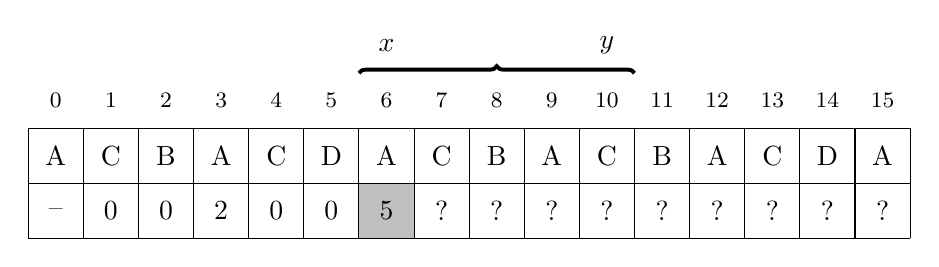
\begin{tikzpicture}[scale=0.7]
\fill[color=lightgray] (6,0) rectangle (7,1);
\draw (0,0) grid (16,2);

\node at (0.5, 1.5) {A};
\node at (1.5, 1.5) {C};
\node at (2.5, 1.5) {B};
\node at (3.5, 1.5) {A};
\node at (4.5, 1.5) {C};
\node at (5.5, 1.5) {D};
\node at (6.5, 1.5) {A};
\node at (7.5, 1.5) {C};
\node at (8.5, 1.5) {B};
\node at (9.5, 1.5) {A};
\node at (10.5, 1.5) {C};
\node at (11.5, 1.5) {B};
\node at (12.5, 1.5) {A};
\node at (13.5, 1.5) {C};
\node at (14.5, 1.5) {D};
\node at (15.5, 1.5) {A};

\node at (0.5, 0.5) {--};
\node at (1.5, 0.5) {0};
\node at (2.5, 0.5) {0};
\node at (3.5, 0.5) {2};
\node at (4.5, 0.5) {0};
\node at (5.5, 0.5) {0};
\node at (6.5, 0.5) {5};
\node at (7.5, 0.5) {?};
\node at (8.5, 0.5) {?};
\node at (9.5, 0.5) {?};
\node at (10.5, 0.5) {?};
\node at (11.5, 0.5) {?};
\node at (12.5, 0.5) {?};
\node at (13.5, 0.5) {?};
\node at (14.5, 0.5) {?};
\node at (15.5, 0.5) {?};

\draw [decoration={brace}, decorate, line width=0.5mm] (6,3.00) -- (11,3.00);

\node at (6.5,3.50) {$x$};
\node at (10.5,3.50) {$y$};


\footnotesize
\node at (0.5, 2.5) {0};
\node at (1.5, 2.5) {1};
\node at (2.5, 2.5) {2};
\node at (3.5, 2.5) {3};
\node at (4.5, 2.5) {4};
\node at (5.5, 2.5) {5};
\node at (6.5, 2.5) {6};
\node at (7.5, 2.5) {7};
\node at (8.5, 2.5) {8};
\node at (9.5, 2.5) {9};
\node at (10.5, 2.5) {10};
\node at (11.5, 2.5) {11};
\node at (12.5, 2.5) {12};
\node at (13.5, 2.5) {13};
\node at (14.5, 2.5) {14};
\node at (15.5, 2.5) {15};

\end{tikzpicture}
\end{center}

Agora podemos calcular os valores subsequentes do array Z de forma eficiente, porque sabemos que $\texttt{s}[0 \ldots 4]$ e $\texttt{s}[6 \ldots 10]$ são iguais. Primeiro, como $\texttt{z}[1] = \texttt{z}[2] = 0$, sabemos imediatamente que também $\texttt{z}[7] = \texttt{z}[8] = 0$:

\begin{center}
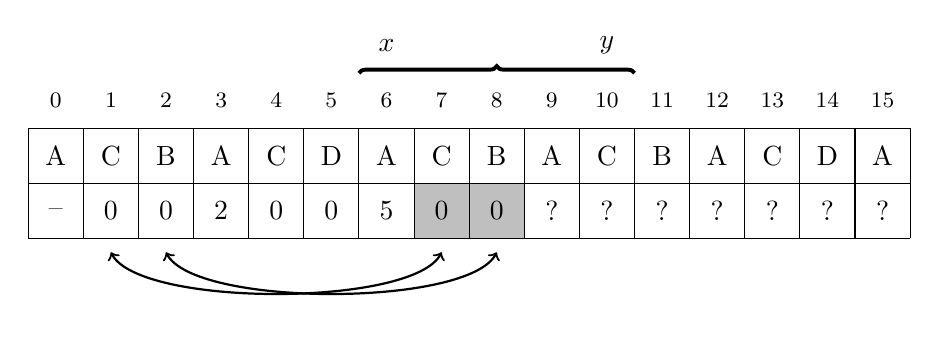
\begin{tikzpicture}[scale=0.7]
\fill[color=lightgray] (7,0) rectangle (9,1);
\draw (0,0) grid (16,2);

\node at (0.5, 1.5) {A};
\node at (1.5, 1.5) {C};
\node at (2.5, 1.5) {B};
\node at (3.5, 1.5) {A};
\node at (4.5, 1.5) {C};
\node at (5.5, 1.5) {D};
\node at (6.5, 1.5) {A};
\node at (7.5, 1.5) {C};
\node at (8.5, 1.5) {B};
\node at (9.5, 1.5) {A};
\node at (10.5, 1.5) {C};
\node at (11.5, 1.5) {B};
\node at (12.5, 1.5) {A};
\node at (13.5, 1.5) {C};
\node at (14.5, 1.5) {D};
\node at (15.5, 1.5) {A};

\node at (0.5, 0.5) {--};
\node at (1.5, 0.5) {0};
\node at (2.5, 0.5) {0};
\node at (3.5, 0.5) {2};
\node at (4.5, 0.5) {0};
\node at (5.5, 0.5) {0};
\node at (6.5, 0.5) {5};
\node at (7.5, 0.5) {0};
\node at (8.5, 0.5) {0};
\node at (9.5, 0.5) {?};
\node at (10.5, 0.5) {?};
\node at (11.5, 0.5) {?};
\node at (12.5, 0.5) {?};
\node at (13.5, 0.5) {?};
\node at (14.5, 0.5) {?};
\node at (15.5, 0.5) {?};


\draw [decoration={brace}, decorate, line width=0.5mm] (6,3.00) -- (11,3.00);

\node at (6.5,3.50) {$x$};
\node at (10.5,3.50) {$y$};


\footnotesize
\node at (0.5, 2.5) {0};
\node at (1.5, 2.5) {1};
\node at (2.5, 2.5) {2};
\node at (3.5, 2.5) {3};
\node at (4.5, 2.5) {4};
\node at (5.5, 2.5) {5};
\node at (6.5, 2.5) {6};
\node at (7.5, 2.5) {7};
\node at (8.5, 2.5) {8};
\node at (9.5, 2.5) {9};
\node at (10.5, 2.5) {10};
\node at (11.5, 2.5) {11};
\node at (12.5, 2.5) {12};
\node at (13.5, 2.5) {13};
\node at (14.5, 2.5) {14};
\node at (15.5, 2.5) {15};


\draw[thick,<->] (7.5,-0.25) .. controls (7,-1.25) and (2,-1.25) .. (1.5,-0.25);
\draw[thick,<->] (8.5,-0.25) .. controls (8,-1.25) and (3,-1.25) .. (2.5,-0.25);
\end{tikzpicture}
\end{center}

Então, como $\texttt{z}[3]=2$, sabemos que $\texttt{z}[9] \ge 2$:

\begin{center}
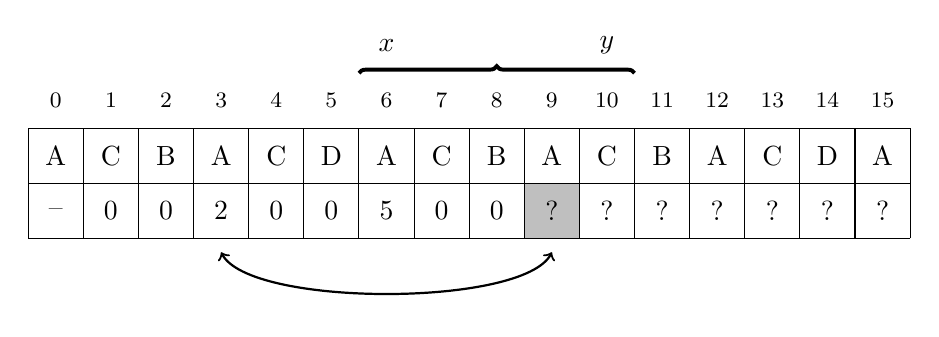
\begin{tikzpicture}[scale=0.7]
\fill[color=lightgray] (9,0) rectangle (10,1);
\draw (0,0) grid (16,2);

\node at (0.5, 1.5) {A};
\node at (1.5, 1.5) {C};
\node at (2.5, 1.5) {B};
\node at (3.5, 1.5) {A};
\node at (4.5, 1.5) {C};
\node at (5.5, 1.5) {D};
\node at (6.5, 1.5) {A};
\node at (7.5, 1.5) {C};
\node at (8.5, 1.5) {B};
\node at (9.5, 1.5) {A};
\node at (10.5, 1.5) {C};
\node at (11.5, 1.5) {B};
\node at (12.5, 1.5) {A};
\node at (13.5, 1.5) {C};
\node at (14.5, 1.5) {D};
\node at (15.5, 1.5) {A};

\node at (0.5, 0.5) {--};
\node at (1.5, 0.5) {0};
\node at (2.5, 0.5) {0};
\node at (3.5, 0.5) {2};
\node at (4.5, 0.5) {0};
\node at (5.5, 0.5) {0};
\node at (6.5, 0.5) {5};
\node at (7.5, 0.5) {0};
\node at (8.5, 0.5) {0};
\node at (9.5, 0.5) {?};
\node at (10.5, 0.5) {?};
\node at (11.5, 0.5) {?};
\node at (12.5, 0.5) {?};
\node at (13.5, 0.5) {?};
\node at (14.5, 0.5) {?};
\node at (15.5, 0.5) {?};

\draw [decoration={brace}, decorate, line width=0.5mm] (6,3.00) -- (11,3.00);

\node at (6.5,3.50) {$x$};
\node at (10.5,3.50) {$y$};


\footnotesize
\node at (0.5, 2.5) {0};
\node at (1.5, 2.5) {1};
\node at (2.5, 2.5) {2};
\node at (3.5, 2.5) {3};
\node at (4.5, 2.5) {4};
\node at (5.5, 2.5) {5};
\node at (6.5, 2.5) {6};
\node at (7.5, 2.5) {7};
\node at (8.5, 2.5) {8};
\node at (9.5, 2.5) {9};
\node at (10.5, 2.5) {10};
\node at (11.5, 2.5) {11};
\node at (12.5, 2.5) {12};
\node at (13.5, 2.5) {13};
\node at (14.5, 2.5) {14};
\node at (15.5, 2.5) {15};

\draw[thick,<->] (9.5,-0.25) .. controls (9,-1.25) and (4,-1.25) .. (3.5,-0.25);
\end{tikzpicture}
\end{center}

No entanto, não temos informações sobre a string após a posição 10, então precisamos comparar as substrings caractere por caractere:

\begin{center}
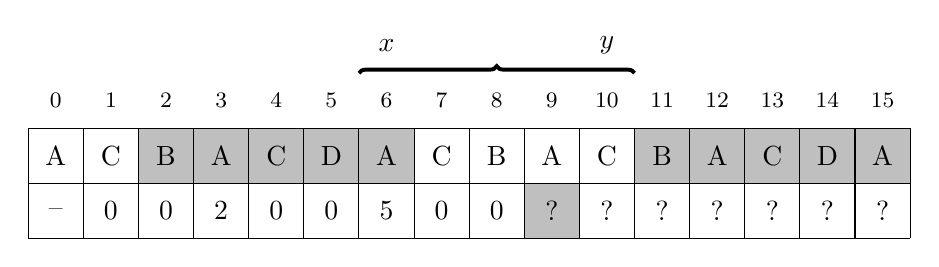
\begin{tikzpicture}[scale=0.7]
\fill[color=lightgray] (9,0) rectangle (10,1);
\fill[color=lightgray] (2,1) rectangle (7,2);
\fill[color=lightgray] (11,1) rectangle (16,2);


\draw (0,0) grid (16,2);

\node at (0.5, 1.5) {A};
\node at (1.5, 1.5) {C};
\node at (2.5, 1.5) {B};
\node at (3.5, 1.5) {A};
\node at (4.5, 1.5) {C};
\node at (5.5, 1.5) {D};
\node at (6.5, 1.5) {A};
\node at (7.5, 1.5) {C};
\node at (8.5, 1.5) {B};
\node at (9.5, 1.5) {A};
\node at (10.5, 1.5) {C};
\node at (11.5, 1.5) {B};
\node at (12.5, 1.5) {A};
\node at (13.5, 1.5) {C};
\node at (14.5, 1.5) {D};
\node at (15.5, 1.5) {A};

\node at (0.5, 0.5) {--};
\node at (1.5, 0.5) {0};
\node at (2.5, 0.5) {0};
\node at (3.5, 0.5) {2};
\node at (4.5, 0.5) {0};
\node at (5.5, 0.5) {0};
\node at (6.5, 0.5) {5};
\node at (7.5, 0.5) {0};
\node at (8.5, 0.5) {0};
\node at (9.5, 0.5) {?};
\node at (10.5, 0.5) {?};
\node at (11.5, 0.5) {?};
\node at (12.5, 0.5) {?};
\node at (13.5, 0.5) {?};
\node at (14.5, 0.5) {?};
\node at (15.5, 0.5) {?};

\draw [decoration={brace}, decorate, line width=0.5mm] (6,3.00) -- (11,3.00);

\node at (6.5,3.50) {$x$};
\node at (10.5,3.50) {$y$};


\footnotesize
\node at (0.5, 2.5) {0};
\node at (1.5, 2.5) {1};
\node at (2.5, 2.5) {2};
\node at (3.5, 2.5) {3};
\node at (4.5, 2.5) {4};
\node at (5.5, 2.5) {5};
\node at (6.5, 2.5) {6};
\node at (7.5, 2.5) {7};
\node at (8.5, 2.5) {8};
\node at (9.5, 2.5) {9};
\node at (10.5, 2.5) {10};
\node at (11.5, 2.5) {11};
\node at (12.5, 2.5) {12};
\node at (13.5, 2.5) {13};
\node at (14.5, 2.5) {14};
\node at (15.5, 2.5) {15};

%\draw[thick,<->] (11.5,-0.25) .. controls (11,-1.25) and (3,-1.25) .. (2.5,-0.25);
\end{tikzpicture}
\end{center}

Acontece que $\texttt{z}[9]=7$, então o novo intervalo $[x,y]$ é $[9,15]$:

\begin{center}
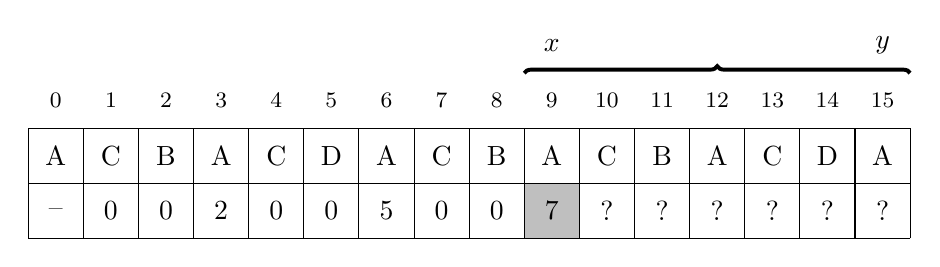
\begin{tikzpicture}[scale=0.7]
\fill[color=lightgray] (9,0) rectangle (10,1);
\draw (0,0) grid (16,2);

\node at (0.5, 1.5) {A};
\node at (1.5, 1.5) {C};
\node at (2.5, 1.5) {B};
\node at (3.5, 1.5) {A};
\node at (4.5, 1.5) {C};
\node at (5.5, 1.5) {D};
\node at (6.5, 1.5) {A};
\node at (7.5, 1.5) {C};
\node at (8.5, 1.5) {B};
\node at (9.5, 1.5) {A};
\node at (10.5, 1.5) {C};
\node at (11.5, 1.5) {B};
\node at (12.5, 1.5) {A};
\node at (13.5, 1.5) {C};
\node at (14.5, 1.5) {D};
\node at (15.5, 1.5) {A};

\node at (0.5, 0.5) {--};
\node at (1.5, 0.5) {0};
\node at (2.5, 0.5) {0};
\node at (3.5, 0.5) {2};
\node at (4.5, 0.5) {0};
\node at (5.5, 0.5) {0};
\node at (6.5, 0.5) {5};
\node at (7.5, 0.5) {0};
\node at (8.5, 0.5) {0};
\node at (9.5, 0.5) {7};
\node at (10.5, 0.5) {?};
\node at (11.5, 0.5) {?};
\node at (12.5, 0.5) {?};
\node at (13.5, 0.5) {?};
\node at (14.5, 0.5) {?};
\node at (15.5, 0.5) {?};

\draw [decoration={brace}, decorate, line width=0.5mm] (9,3.00) -- (16,3.00);

\node at (9.5,3.50) {$x$};
\node at (15.5,3.50) {$y$};


\footnotesize
\node at (0.5, 2.5) {0};
\node at (1.5, 2.5) {1};
\node at (2.5, 2.5) {2};
\node at (3.5, 2.5) {3};
\node at (4.5, 2.5) {4};
\node at (5.5, 2.5) {5};
\node at (6.5, 2.5) {6};
\node at (7.5, 2.5) {7};
\node at (8.5, 2.5) {8};
\node at (9.5, 2.5) {9};
\node at (10.5, 2.5) {10};
\node at (11.5, 2.5) {11};
\node at (12.5, 2.5) {12};
\node at (13.5, 2.5) {13};
\node at (14.5, 2.5) {14};
\node at (15.5, 2.5) {15};

% \draw[thick,<->] (9.5,-0.25) .. controls (9,-1.25) and (4,-1.25) .. (3.5,-0.25);
\end{tikzpicture}
\end{center}

Após isso, todos os valores restantes do array Z podem ser determinados usando as informações já armazenadas no array Z:

\begin{center}
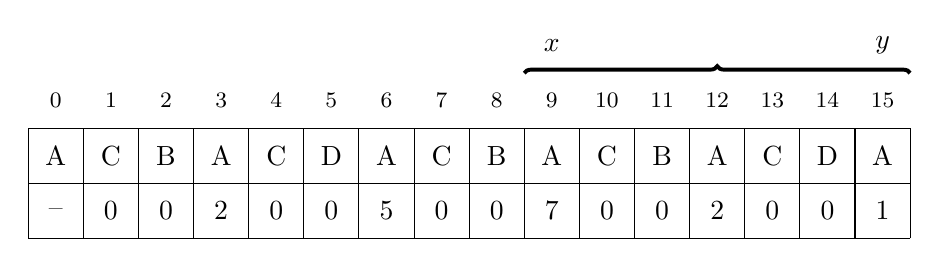
\begin{tikzpicture}[scale=0.7]
\draw (0,0) grid (16,2);

\node at (0.5, 1.5) {A};
\node at (1.5, 1.5) {C};
\node at (2.5, 1.5) {B};
\node at (3.5, 1.5) {A};
\node at (4.5, 1.5) {C};
\node at (5.5, 1.5) {D};
\node at (6.5, 1.5) {A};
\node at (7.5, 1.5) {C};
\node at (8.5, 1.5) {B};
\node at (9.5, 1.5) {A};
\node at (10.5, 1.5) {C};
\node at (11.5, 1.5) {B};
\node at (12.5, 1.5) {A};
\node at (13.5, 1.5) {C};
\node at (14.5, 1.5) {D};
\node at (15.5, 1.5) {A};

\node at (0.5, 0.5) {--};
\node at (1.5, 0.5) {0};
\node at (2.5, 0.5) {0};
\node at (3.5, 0.5) {2};
\node at (4.5, 0.5) {0};
\node at (5.5, 0.5) {0};
\node at (6.5, 0.5) {5};
\node at (7.5, 0.5) {0};
\node at (8.5, 0.5) {0};
\node at (9.5, 0.5) {7};
\node at (10.5, 0.5) {0};
\node at (11.5, 0.5) {0};
\node at (12.5, 0.5) {2};
\node at (13.5, 0.5) {0};
\node at (14.5, 0.5) {0};
\node at (15.5, 0.5) {1};

\draw [decoration={brace}, decorate, line width=0.5mm] (9,3.00) -- (16,3.00);

\node at (9.5,3.50) {$x$};
\node at (15.5,3.50) {$y$};


\footnotesize
\node at (0.5, 2.5) {0};
\node at (1.5, 2.5) {1};
\node at (2.5, 2.5) {2};
\node at (3.5, 2.5) {3};
\node at (4.5, 2.5) {4};
\node at (5.5, 2.5) {5};
\node at (6.5, 2.5) {6};
\node at (7.5, 2.5) {7};
\node at (8.5, 2.5) {8};
\node at (9.5, 2.5) {9};
\node at (10.5, 2.5) {10};
\node at (11.5, 2.5) {11};
\node at (12.5, 2.5) {12};
\node at (13.5, 2.5) {13};
\node at (14.5, 2.5) {14};
\node at (15.5, 2.5) {15};

\end{tikzpicture}
\end{center}

\subsubsection{Usando o array Z}

Muitas vezes, é uma questão de preferência usar hashing de string ou o algoritmo Z. Ao contrário do hashing, o algoritmo Z sempre funciona e não há risco de colisões. Por outro lado, o algoritmo Z é mais difícil de implementar e alguns problemas só podem ser resolvidos usando hashing.

Como exemplo, considere novamente o problema de casamento de padrão, onde nossa tarefa é encontrar as ocorrências de um padrão $p$ em uma string $s$. Já resolvemos este problema de forma eficiente usando hashing de string, mas o algoritmo Z fornece outra maneira de resolver o problema.

Uma ideia usual no processamento de strings é construir uma string que consiste em múltiplas strings separadas por caracteres especiais. Neste problema, podemos construir uma string $p$\texttt{\#}$s$, onde $p$ e $s$ são separados por um caractere especial \texttt{\#} que não ocorre nas strings. O array Z de $p$\texttt{\#}$s$ nos diz as posições onde $p$ ocorre em $s$, porque tais posições contêm o comprimento de $p$.

Por exemplo, se $s=$\texttt{HATTIVATTI} e $p=$\texttt{ATT}, o array Z é o seguinte:

\begin{center}
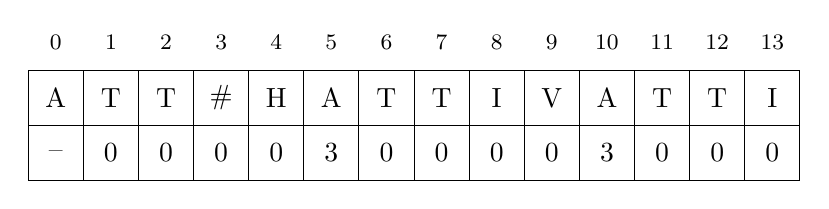
\begin{tikzpicture}[scale=0.7]
\draw (0,0) grid (14,2);

\node at (0.5, 1.5) {A};
\node at (1.5, 1.5) {T};
\node at (2.5, 1.5) {T};
\node at (3.5, 1.5) {\#};
\node at (4.5, 1.5) {H};
\node at (5.5, 1.5) {A};
\node at (6.5, 1.5) {T};
\node at (7.5, 1.5) {T};
\node at (8.5, 1.5) {I};
\node at (9.5, 1.5) {V};
\node at (10.5, 1.5) {A};
\node at (11.5, 1.5) {T};
\node at (12.5, 1.5) {T};
\node at (13.5, 1.5) {I};

\node at (0.5, 0.5) {--};
\node at (1.5, 0.5) {0};
\node at (2.5, 0.5) {0};
\node at (3.5, 0.5) {0};
\node at (4.5, 0.5) {0};
\node at (5.5, 0.5) {3};
\node at (6.5, 0.5) {0};
\node at (7.5, 0.5) {0};
\node at (8.5, 0.5) {0};
\node at (9.5, 0.5) {0};
\node at (10.5, 0.5) {3};
\node at (11.5, 0.5) {0};
\node at (12.5, 0.5) {0};
\node at (13.5, 0.5) {0};

\footnotesize
\node at (0.5, 2.5) {0};
\node at (1.5, 2.5) {1};
\node at (2.5, 2.5) {2};
\node at (3.5, 2.5) {3};
\node at (4.5, 2.5) {4};
\node at (5.5, 2.5) {5};
\node at (6.5, 2.5) {6};
\node at (7.5, 2.5) {7};
\node at (8.5, 2.5) {8};
\node at (9.5, 2.5) {9};
\node at (10.5, 2.5) {10};
\node at (11.5, 2.5) {11};
\node at (12.5, 2.5) {12};
\node at (13.5, 2.5) {13};
\end{tikzpicture}
\end{center}

As posições 5 e 10 contêm o valor 3, o que significa que o padrão \texttt{ATT} ocorre nas posições correspondentes de \texttt{HATTIVATTI}.

A complexidade de tempo do algoritmo resultante é linear, pois é suficiente construir o array Z e percorrer seus valores.

\subsubsection{Implementação}

Aqui está uma implementação curta do algoritmo Z que retorna um vetor que corresponde ao array Z.

\begin{lstlisting}
vector<int> z(string s) {
    int n = s.size();
    vector<int> z(n);
    int x = 0, y = 0;
    for (int i = 1; i < n; i++) {
        z[i] = max(0,min(z[i-x],y-i+1));
        while (i+z[i] < n && s[z[i]] == s[i+z[i]]) {
            x = i; y = i+z[i]; z[i]++;
        }
    }
    return z;
}
\end{lstlisting}
